\section{Introduction}
\label{sec:introduction}
\subsection{Background}
\subsubsection{Stewart Platform}
\paragraph{}A Stewart platform is a platform with six degrees of freedom (DOF)
\cite{stewart1965platform}. It comprises a triangular/rectangular/circular plane called the platform, of which each of the attachments to the platform is connected through a three-axis joint to one of three legs.
A Stewart platform is shown in Fig.1.1.
\begin{center}
	\begin{figure}[!h]
	\centering
	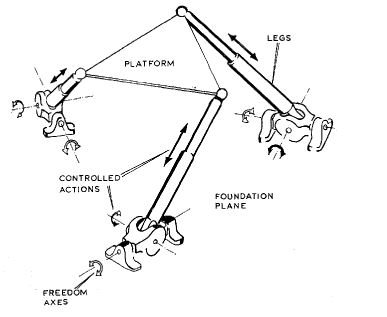
\includegraphics{Figures/Fig1}
	\caption{General arrangement}
	\end{figure}
\end{center}
\paragraph{}Each leg of the Stewart platform is connected to the ground by a two-axis joint and is provided with controllable means for extending its length.
%\begin{enumerate}
%\item Use of two hydraulic jacks
%\item Screw Jacks
%\item Rotary actuator
%\item Levers
%\item Linear co-ordinate control
%\item Strength
%\end{enumerate}
%\paragraph{}These shall be discussed in detail at a later stage.
\subparagraph{Application}
\paragraph{}The six DOF Stewart Platform provides an elegant design for simulating flight conditions that can be used in safe training of pilots
\cite{stewart1965platform}.
\subsubsection{Wind Tunnel}
\paragraph{}
A wind tunnel is a large tube with air moving inside. This movement of air is usually done by powerful fans. The tunnel is used to copy the actions of an object in flight thus allowing
to obtain the components that better define this interaction, forces and moments \cite{morris_force_2010}.
\paragraph{} The first wind tunnel was built by
Francis Wenham in 1871. However, it was the Wright Brothers who were the first to show the value of the wind tunnel in aerodynamic design with their 1902 wind tunnel.  The Wright Brothers’ wind tunnel was largely made of wood, with a glass window on the top to look down through and see the force balance, from which the
lift and drag forces could be read. The wind tunnel was powered by a fan driven off a natural gas fueled engine. Their tunnel was square of 16" by 16"(about 407mm by 407mm), and 6 foot long (about 1829mm), with a maximum test speed of 35 mph (about 56 km/h) \cite{fernandes_design_nodate}.
%\begin{center}
	\begin{figure}[!h]
	%\centering
	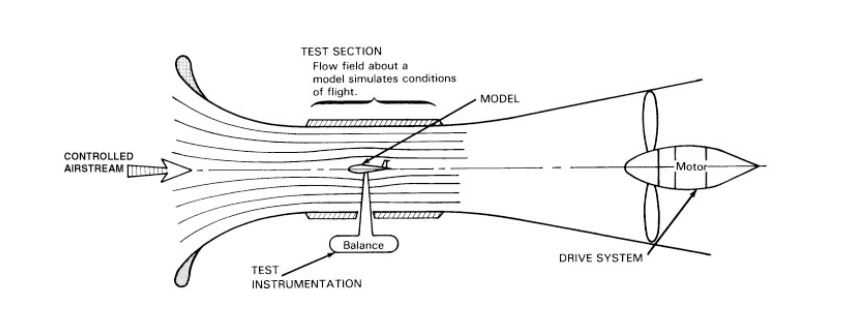
\includegraphics{Figures/Fig2}
	\caption{Diagram of a typical wind tunnel}
	\end{figure}
%\end{center}
\paragraph{}
Later in the early 20th century in Europe, the main users of wind tunnels were Gustave Eiffel in France and Ludwig Prandtl in Germany. Prandtl built the first closed circuit wind tunnel in 1908.
%\paragraph{}Closed circuit wind tunnels are characterized by the recirculation of the airflow with with very minimal exchange with the exterior. Open circuit wind tunnels on the other hand, have an airflow that follows a straight path and flows to the contracted zone where the test section is located and then passes through a diffuser, a fan section
%and an exhaust.
By the 1940’s supersonic wind tunnels were in use. In 1972 a cryogenic wind tunnel was built at NASA Langley by injecting liquid nitrogen into the wind tunnel to cool the gas. This lowered the viscosity and increased the Reynolds number, and this tunnel had the capability to match Reynolds and Mach numbers simultaneously up to Mach 1.2. 
\cite{fernandes_design_nodate}
\paragraph{}Today the largest wind tunnel in the world is the National Full-Scale Aerodynamics Complex at NASA's Ames Research Center, which has a test section of cross section 80 ft by 100 ft (24 m x 31 m). The types of instruments in common use in wind tunnels include boundary layer rakes, tufts, pitot tubes, pressure sensitive paint, smoke, and static pressure taps.
\begin{center}
\begin{figure}[!h]
	\centering
	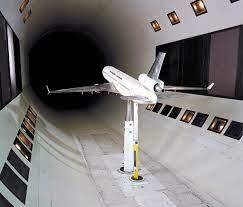
\includegraphics{Figures/Fig3}
	\caption{NASA wind tunnels used to test new airplane designs}
\end{figure}
\end{center}
\paragraph{}NASA uses wind tunnels to test scale models of aircraft and spacecraft. Wind tunnels help NASA to test ideas of making airplanes better and safer. They are also used to help engineers in designing spacecraft that will work in other planets such as mars - the wind tunnel can be used to simulate objects in an atmosphere that's thinner than ours e.g. an atmosphere that's exactly like the Martian atmosphere. NASA has wind tunnels of different types and sizes. Some are low-speed wind tunnels, others are hypersonic i.e. they are made to carry out tests at 4,000 mph (6437 kph).
\begin{center}
     %&\vspace*{-4.0cm}
    \begin{figure}[!h]
\centering
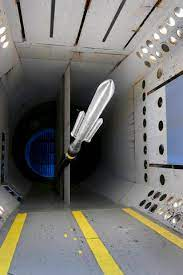
\includegraphics{Figures/Fig4}
\caption{NASA wind tunnels used to test the design of heavy-lift rocket}
\end{figure}
\end{center}
%\paragraph{}Wind tunnels are used to measure the aerodynamic forces on airplanes, wings, cars, trucks, bridges, and buildings, they can also be used to measure the
%aerodynamic forces on sports balls, partially open valves, and anything else that can be mounted on the mounting sting. Wind tunnels are an effective tool used by engineers in determining the various aerodynamic loads due to movement of these vessels during the development process.
%For wind tunnel testing with scale models to be applicable to the aerodynamics of the full-scale test object, conditions of dynamic similarity must be met.
\subsubsection{Force Balance and Load Sensors}
\paragraph{}A force balance is a device used to take direct measurement of forces and torques acting on the model that is being tested in the wind tunnel. The need for force balances arises due to the necessity of having maximum load capability in all measuring components along with the accuracy for measuring minimum loads. 
\cite{fernandes_design_nodate}
\paragraph{}The force balance is intended to be built as simple and accessible as possible. Thus, the development of a three-component balance will be considered.

\paragraph{}Several load measurement devices have to be connected to the main structure in order to measure and obtain the results and so making it fully operational. This project looks to employ electrical load measurement techniques. Strain gauges will be used.
%Force balances can be external or internal. In external force balances the test section lies outside of the wind tunnel test section, whereas in internal force balances the balance is inside the model itself connecting the model to the support structure.

%\paragraph{}Several different types of external force balances are available for wind tunnel use
%\cite{morris_force_2010}:
%\begin{enumerate}
%\item Wire
%\item Platform
%\item Yoke
%\item Pyramidal
%\end{enumerate}
%\paragraph{}The different kinds of internal balances can be made based on:
%1 the type of transducer i.e. strain gauge or piezoelectric balance.
%2 shape i.e. box balance and sting balance

\subsection{Problem statement}
\paragraph{}Simulation and analysis of scaled models is an important step in the development of aircrafts, vehicles and other machines . Such analysis provides aerodynamic peformance data that can be used to inform any modifications or improvements e.g. in aircrafts and vehicles to make them more efficient and safer. One such method that is used to perform aerodynamic performance evaluation is the wind tunnel, which can be low speed or high speed, used in conjuction with sensors for data aquisition by a computer. External or internal six-component force balances are also used. Another such technology that can be used for this purpose is the Stewart platform, which can be used to predict behaviour of vehicles and aircrafts in the actual environment.
\paragraph{}Whereas the wind tunnel gives very accurate results, it is expensive to build and use. Also, some objects require complex maneuver simulations to imitate the actual movements in air. There is therefore the need for dynamic positioning of objects in the wind tunnel.

\paragraph{}This project proposal, therefore, presents the development of a 3-component external force moment-balance to stand as a simple and economical alternative to the existing commercial solutions. The force balance should be able to measure lift, drag and pitching moment in small models and will be used with a generic low speed wind tunnel which is already available. The proposal also presents the design of a six-degrees-of-freedom Stewart platform to simulate the different movemnets of objects.
\subsection{Objectives}
\subsubsection{Main Objective}
\paragraph{} To develop an external Stewart platform force balance for a low speed wind tunnel 
\subsubsection{Specific Objectives}
\begin{enumerate}
\item To design and fabricate a six-degrees-of-freedom Stewart platform
\item To develop a force balance for the Stewart platform
\item To obtain forces and moments from a test model
\end{enumerate}
\subsection{Justification of the study}
\paragraph{} In a large percentage of cases the measurement of forces and moment expereince by a model during wind ttunnel testing is critical. To achieve this in a cost sustinable way as well as well as allowing the dynamic positioning of model for different test cases is important for development of aerodynamic bodies and parts. In many cases where both these goals are achieved it results in expensive and har to maintain devices or integrated wind tunnels. Our project will be going into the development of a six-degrees-of-freedom Stewart Platform and three-component Force balance. We will use the low speed wind tunnel that is currently available at the fluids laboratory.
